% C094 precise confocal ellipse/hyperbola diagram
% E: x^2/16+y^2/12=1 ; H: x^2-y^2/3=1 ; F1=(-2,0),F2=(2,0)
% Intersections: (+/-2, +/-3). Geometry controlled by exact equations.
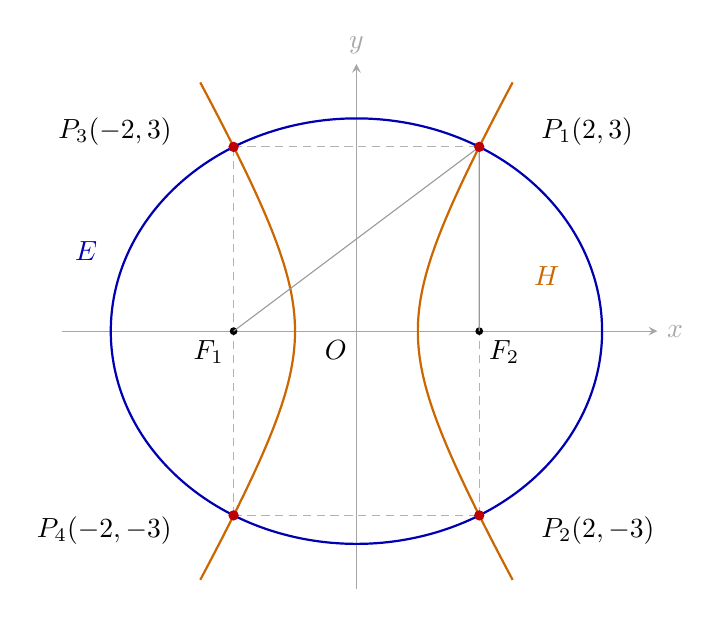
\begin{tikzpicture}[scale=0.78,>=stealth]
  \draw[->,gray!70] (-4.8,0)--(4.9,0) node[right] {$x$};
  \draw[->,gray!70] (0,-4.2)--(0,4.35) node[above] {$y$};
  \draw[thick,blue!70!black,domain=0:360,samples=220,smooth,variable=\t]
      plot ({4*cos(\t)},{sqrt(12)*sin(\t)});
  \draw[thick,orange!80!black,domain=-4.05:4.05,samples=100,smooth,variable=\t]
      plot ({sqrt(1+\t*\t/3)},{\t});
  \draw[thick,orange!80!black,domain=-4.05:4.05,samples=100,smooth,variable=\t]
      plot ({-sqrt(1+\t*\t/3)},{\t});
  \draw[densely dashed,gray!60] (-2,-3)--(-2,3) (2,-3)--(2,3)
                                 (-2,3)--(2,3) (-2,-3)--(2,-3);
  \fill (-2,0) circle (1.8pt) node[below left] {$F_1$};
  \fill (2,0) circle (1.8pt) node[below right] {$F_2$};
  \draw[thin,gray!80] (-2,0)--(2,3)--(2,0);
  \foreach \x/\y in {2/3,2/-3,-2/3,-2/-3} {
    \fill[red!75!black] (\x,\y) circle (2.4pt);
  }
  \node[anchor=west] at (2.85,3.25) {$P_1(2,3)$};
  \node[anchor=west] at (2.85,-3.25) {$P_2(2,-3)$};
  \node[anchor=east] at (-2.85,3.25) {$P_3(-2,3)$};
  \node[anchor=east] at (-2.85,-3.25) {$P_4(-2,-3)$};
  \node[blue!70!black] at (-4.4,1.3) {$E$};
  \node[orange!80!black] at (3.1,0.9) {$H$};
  \node[below left] at (0,0) {$O$};
\end{tikzpicture}
